\chapter{Implantation De Le Loi De Commande}
      
       
 
 
\addcontentsline{toc}{chapter}{Implantation De Le Loi De Commande}
 \section{Calcul D’un Observateur Minimal Identité}

 \subsection{Le modèle linéarisé est-il observable ?}
 
 Pour voir est ce que le système étudier est observable   on va calculer la matrice \\
 Méthode analytique :\\\\
      $obs$=$\begin{bmatrix}
      C & CA & CA^{2}
      \end{bmatrix}^{T}$\\\\
      
      $obs$=$\begin{bmatrix}
      0 & 0 & 0 \\
      0 & 0 & 0 \\
      0 & 0 & 0 \\
      \end{bmatrix}$
 
 %%%%%%%%%%%copmpleter%%%%%%%%
 
 \subsection{Calcul Du Nouveau Observateur identité }
Constitution de l'observateur minimale identité\\\\
$A$=$\begin{bmatrix}
-0.0092 & 0.0092 & 0 \\
0.0092 & -0.0198 & 0.0106\\
0 & 0.0106 & 0.0486\\
\end{bmatrix}$\\\\
Séparation de la matrice A 

$A_{11}=\begin{bmatrix}
-0.0092
\end{bmatrix}
\quad ;
A_{21}=\begin{bmatrix}
0.0092\\
0
\end{bmatrix}$\\\\


$A_{11}=\begin{bmatrix}
0.0092 & 0
\end{bmatrix}
\quad ;
A_{22}=\begin{bmatrix}
-0.0198 & 0.0106 \\
0.0106 & 0.0486
\end{bmatrix}$\\\\
 


\begin{equation}
\left\{\begin{matrix}
\dot{s}(t)=Fs(t)+(FG-GA_{11}+A_{21})y(t)+(B_{2}-GB_{1}u(t))\\
 x^(t)=s(t)+Gy(t)\\
\end{matrix}\right.
\end{equation}   
talque\\ 
$F$=$A_{22}-GA_{12}$\\\\
alors on a \\\\
$\begin{bmatrix}
f_{11} & f_{12}\\
f_{21} & f_{22}\\
\end{bmatrix}
\quad=
\begin{bmatrix}
1 & 1\\
0 & 1\\
\end{bmatrix}
\quad-
\begin{bmatrix}
g1\\
g2\\
\end{bmatrix}
\quad
\begin{bmatrix}
0.0092 & 0
\end{bmatrix}$\\\\

alors on aura \\\\
$F=
\begin{bmatrix}
f_{11} & f_{12}\\
f_{21} & f_{22}\\
\end{bmatrix}
\quad=
\begin{bmatrix}
(1-0.0092g_{1}) & 1\\
(-0.0092g_{2}) && 1\\
\end{bmatrix}$\\\\

puis en calcule  le déterminent de cette matrice puis on va faire l'identification avec le polynôme désiré\\\\

$det(\lambda I-F)= 2-0.0092g_{1}\lambda-0.0092_{g2}$\\

$P_{désiré}=(\lambda+0.04)(\lambda+0.05)\\
           =\lambda^{2}+0.09\lambda+0.002$\\\\


par identification on trouve:\\\\

$G=\begin{bmatrix}
216\\
0.217\\
\end{bmatrix}
\quad
F=\begin{bmatrix}
-0.009872 & 1\\
 0.001996 & 1\\
\end{bmatrix}$\\\\

$Calcule De G_{tild} et H_{tild}$:\\\\

$G_{tild}=FG-GA_{11}+A_{21}
\quad\\\\
G_{tild}=\begin{bmatrix}
-1.91\\
 0.6481\\
\end{bmatrix}$\\\\
$B_{11}=\begin{bmatrix}
64.9351
\end{bmatrix}
\quad 
B_{21}=\begin{bmatrix}
0\\
0
\end{bmatrix}$


$H_{tild}=B_{21}G-GB_{11}
\quad\\\\
G_{tild}=\begin{bmatrix}
-1.91\\
 0.6481\\
\end{bmatrix}\\\\$







           
           



  
 
 
 \subsection{Insertion Dans Notre  Schéma Simulink l’observateur sous la forme d’un bloc State-Space.}
 
 
 \subsection{Étude en boucle fermer  }
  \subsubsection{ Vérification que les états estimés convergent vers les états réels du système linéarisé
lorsque les hauteurs initiales sont non nulles.}
  \subsubsection{Évaluation la vitesse de convergence.}
  
  
 \subsection{Réalisation Du Bouclage Déterminé Précédemment En Utilisant les états estimés (cf. figure 4.1).} 
 
\begin{center}
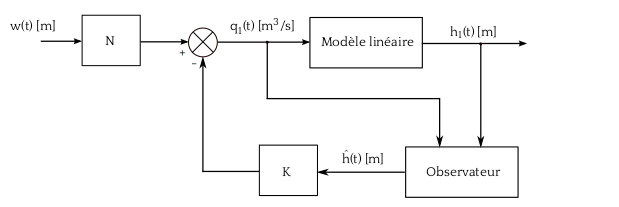
\includegraphics[scale=0.5]{fig3.png}
\captionof{figure}{\textit{ Observateur.}}
\label{fig3} 
\end{center}
 
 
 \subsection{Évaluation De  L’influence des Conditions Initiales}
 
 
 \subsection{Tracer  Des 3 courbes}
  \subsubsection{Schéma Simulink de l’asservissement par retour de sortie}
  \subsubsection{Évolution de l’erreur d’estimation;}
  \subsubsection{Évolution de la consigne et de la sortie mesurée}
  
 \section{Bruit Sur La Sortie Mesurée}

  \subsection{Que constate-t-on sur la sortie du système et sur les états estimés pour le schéma pour le schéma de commande précédent?}
  \subsection{Que constate-t-on sur la sortie du système et sur les états estimés pour le schéma pour le schéma de commande précédent?}
   \subsubsection{Quel est sont effet } 
  
  \section{Expliquez le phénomène observé lors des deux dernières questions en vous basant sur une analyse fréquen-tielle des observateurs.} 